\chapter{Analyzing the genetic structure of populations: a Bayesian approach}

Our review of Nei's $G_{st}$ and Weir and Cockerham's $\theta$
illustrated two important principles:

\begin{enumerate}

\item It's essential to distinguish {\it parameters} from {\it
  estimates}. {\it Parameters} are the things we're really interested
  in, but since we always have to make inferences about the things
  we're really interested in from limited data, we have to rely on
  {\it estimates} of those parameters.\index{parameter}\index{estimate}

\item This means that we have to identify the possible sources of
  sampling error in our estimates and to find ways of accounting for
  them. In the particular case of Wright's $F$-statistics we saw that,
  there are two sources of sampling error: the error associated with
  sampling only some individuals from a larger universe of individuals
  within populations ({\it statistical sampling\/}) and the error
  associated with sampling only some populations from a larger
  universe of populations ({\it genetic sampling\/}).\footnote{The
  terms ``statistical sampling'' and ``genetic sampling'' are due to
  Weir~\cite{Weir-1996}.}\index{sampling!statistical}\index{sampling!genetic}

\end{enumerate}

\noindent It shouldn't come as any surprise that there is a Bayesian
way to do what I've just described. As I hope to convince you, there
are some real advantages associated with doing so.

\section*{The Bayesian model}

I'm not going to provide all of the gory details on the Bayesian
model. If you're interested you can find most of them in my lecture
notes from the \htmladdnormallink{Summer Institute in Statistical
  Genetics}{http://darwin.eeb.uconn.edu/summer-institute/summer-institute.html}
last summer.\footnote{Or you can read Holsinger and
  Wallace~\cite{Holsinger-Wallace-2004}, which I've linked to from the
  course web site.} In fact, I'm only going to describe two pieces of
the model.\footnote{The good news is that to do the Bayesian analyses
  in this case, you don't have to write any {\tt JAGS} code. I'll
  provide the code, Alternatively, you can use a standalone program,
  {\tt Hickory}, that will do the analysis for your, provided you're
  willing to get your data into a format that {\tt Hickory}
  recognizes.} First, a little notation:
\begin{eqnarray*}
n_{11,i} &=& \hbox{\# of $A_1A_1$ genotypes} \\
n_{12,i} &=& \hbox{\# of $A_1A_2$ genotypes} \\
n_{22,i} &=& \hbox{\# of $A_2A_2$ genotypes} \\
i         &=& \hbox{population index} \\
I         &=& \hbox{number of populations} \\
\end{eqnarray*}
These are the data we have to work with. The corresponding genotype
frequencies are
\begin{eqnarray*}
x_{11,i} &=& p_{i}^2 + fp_{i}(1-p_{i}) \\
x_{12,i} &=& 2p_{i}(1-p_{i})(1-f) \\
x_{22,i} &=& (1-p_{i})^2 + fp_{i}(1-p_{i})
\end{eqnarray*}
So we can express the likelihood of our sample as a product of
multinomial probabilities
\[
P({\bf n}|{\bf p},f) \propto \prod_{i=1}^I x_{11,i}^{n_{11,i}}
x_{12,i}^{n_{12,i}} x_{22,i}^{n_{22,i}} \quad .
\]

To complete the Bayesian model, all we need are some appropriate
priors. Specifically, we so far haven't done anything to describe the
variation in allele frequency among populations. Suppose that the
distribution of allele frequencies among populations is
well-approximated by a Beta distribution.\index{Beta
  distribution}\index{allele frequency distribution} A Beta
distribution is convenient for many reasons, and it is quite
flexible. Don't worry about what the formula for a Beta distribution
looks like. All you need to know is that it has two parameters and
that if these parameters are $\pi$ and $\theta$, we can set things up
so that
\begin{eqnarray*}
\mbox{E}(p_{ik}) &=& \pi \\
\mbox{Var}(p_{ik}) &=& \pi(1-\pi)\theta
\end{eqnarray*}
Thus $\pi$ corresponds to $\bar p$ and $\theta$ corresponds to
$F_{st}$.\footnote{For any of you who happen to be familiar with the
usual parameterization of a Beta distribution, this parameterization
corresponds to setting $\nu = ((1-\theta)/\theta)\pi$ and $\omega =
((1-\theta)/\theta)(1-\pi)$.} Figure~\ref{fig:beta} illustrates the
shape of the Beta distribution for different choices of $\pi$ and
$\theta$. To complete the Bayesian model we need only to specify
priors on $\pi$, $f$, and $\theta$. In the absence of any prior
knowledge about the parameters, a uniform prior on [0,1]\footnote{{\tt
dunif(0,1)} in {\tt JAGS} notation} is a natural choice.
\begin{figure}
\resizebox{\textwidth}{!}{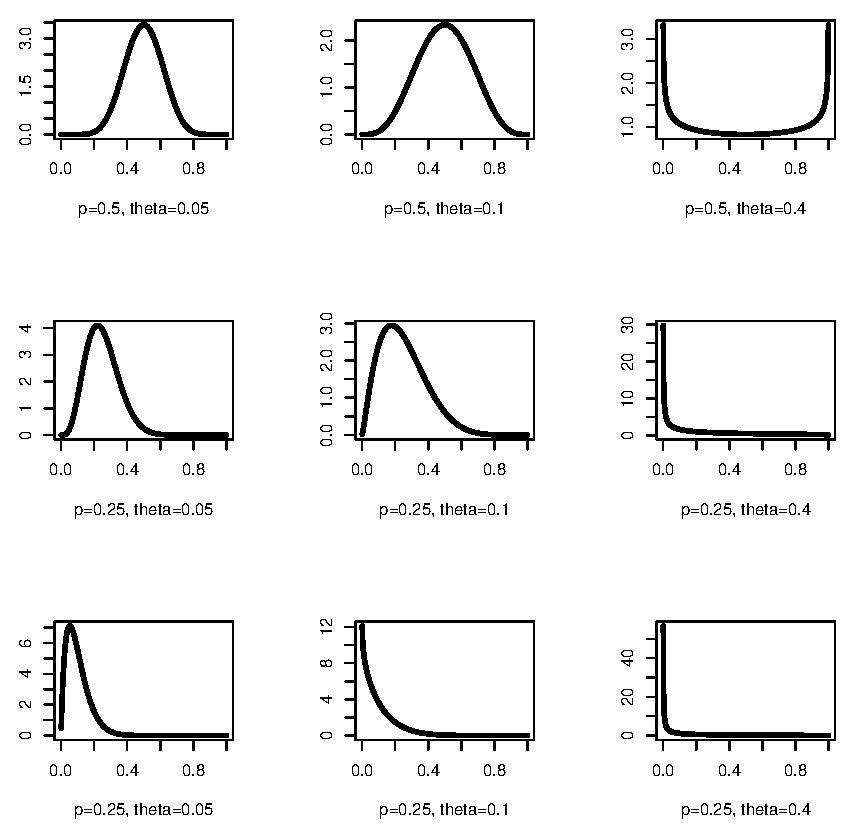
\includegraphics{beta-distribution.eps}}
\caption{Shapes of the Beta distribution for different choices of
  $\pi$ and $\theta$. In the figure captions ``p'' corresponds to $\pi$,
  and ``theta'' corresponds to $\theta$.}\label{fig:beta}
\end{figure}

\subsection*{The {\it Isotoma petraea} example}

Here's the {\tt JAGS} code to estimate $f$ and $\theta$:
\begin{verbatim}
model {
   ## genotype frequencies
   ##
   for (i in 1:n.pops) {
     for (j in 1:n.loci) {
       x[i,j,1] <- p[i,j]*p[i,j] + f*p[i,j]*(1-p[i,j])
       x[i,j,2] <- 2*(1-f)*p[i,j]*(1 - p[i,j])
       x[i,j,3] <- (1-p[i,j])*(1-p[i,j]) + f*p[i,j]*(1-p[i,j])
     }
   }

   ## likelihood
   ##
   for (i in 1:n.pops) {
     for (j in 1:n.loci) {
       n[i,j,1:3] ~ dmulti(x[i,j,], N[i,j])
     }
   }

   ## priors
   ##
   ## allele frequencies within populations
   ##
   for (i in 1:n.pops) {
     for (j in 1:n.loci) {
       p[i,j] ~ dbeta(alpha, beta)
     }
   }
   ## inbreeding coefficient within populations
   ##
   f ~ dunif(0, 1)

   ## theta (Fst)
   ##
   theta ~ dunif(0,1)

   ## pi
   ##
   for (i in 1:n.loci) {
     pi[j] ~ dunif(0,1)
   }

   ## parameters of the beta distribution
   ## the weird constraints are to ensure that both of them
   ## lie in [1, 1.0e4]
   ##
   for (i in 1:n.loci) {
     alpha[i] <- max(1, min(((1-theta)/theta)*pi[i], 1.0e4))
     beta[i]  <- max(1, min(((1-theta)/theta)*(1-pi[i]), 1.0e4))
   }
}
\end{verbatim}

You'll also find an {\tt R} script that calls this code. The relevant
function has the very creative name of {\tt analyze.data()}. It
requires data in a very particular format, namely a list that consists
of four named elements:

\begin{enumerate}

\item {\tt n.pops}: The number of populations in the sample.

\item {\tt n.loci}: The number of loci scored in the sample.

\item {\tt n}: A {\tt n.pops}$\times${\tt n.loci}$\times${\tt 3}
  matrix of genotype counts where in the final dimension the first
  entry corresponds to the number of $A1A1$ homozygotes, the second
  entry corresponds to the number of $A1A2$ heterozygotes, and the
  third entry corresponds to the number of $A2A2$ homozygotes.

\item {\tt N}: An {\tt n.pops}$\times${\tt n.loci} matrix of sample
  sizes at each locus. This could be calculated automatically by {\tt
    analyze.data()}, but I haven't written that code yet.

\end{enumerate}

It's not too hard to get data into that format. {\tt f-statistics.R}
also provides a set of functions to construct that list from a CSV
file in which each line corresponds with an individual, the first
column ({\tt pop}) is the population from which that individual was
collected, and the remaining columns are the genotype (scored as 0, 1,
2) of the individual at a particular locus.

The {\it Isotoma petraea\/} data come to us in a somewhat different
format, so there's also a script that constructs the necessary input
list and calls {\tt analyze.data()}. If you look at the code, you'll
see that I've specified {\tt n.chains=5}. That allows me to check
convergence by looking at {\tt Rhat}. If you run the code, here's what
you'll get (except for MCMC error):
\begin{verbatim}
> print(fit)
Inference for Bugs model at "f-statistics.txt", fit using jags,
 5 chains, each with 30000 iterations (first 25000 discarded), n.thin = 5
 n.sims = 5000 iterations saved
         mu.vect sd.vect   2.5%    25%    50%    75%  97.5%  Rhat n.eff
f          0.527   0.097  0.327  0.464  0.533  0.595  0.698 1.001  5000
theta      0.112   0.051  0.024  0.076  0.108  0.143  0.223 1.003  3000
deviance  46.679   4.848 38.924 43.096 46.095 49.594 57.610 1.001  3900

For each parameter, n.eff is a crude measure of effective sample size,
and Rhat is the potential scale reduction factor (at convergence, Rhat=1).

DIC info (using the rule, pD = var(deviance)/2)
pD = 11.8 and DIC = 58.4
DIC is an estimate of expected predictive error (lower deviance is better).
\end{verbatim}

It's easy to modify the code to consider two special cases:

\begin{itemize}

\item $f=0$: This corresponds to the case when genotypes within
  populations are in Hardy-Weinberg proportions. Implemented in {\tt
    f-statistics-f0.txt}.

\item $\theta=0$: This corresponds to the case when population allele
  frequencies are identical across populations, i.e., there is no
  genetic differentiation. Implemented in {\tt f-statistics-t0.txt}

\end{itemize}
Before we go any further though and start comparing these models,
remember when I said that you need to be careful about using the DIC
reported from {\tt R2jags}? This is one of those cases where I don't
trust it. Why? Because I calculated it from scratch and got a very
different result:\footnote{Just include {\tt DIC=TRUE} in the
  arguments to {\tt analyze.data()} and you'll get a printout of these
  results.}
\begin{verbatim}
Dbar: 46.5
Dhat: 40.7
pD:   5.8
DIC:  52.3
\end{verbatim}
If you compare these results to what's reported from {\tt R2jags},
you'll see that {\tt Dbar} in my calculation corresponds to the
average deviance in the {\tt R2jags} output.\footnote{Except for
  rounding error.} That's because they're both calculated as -2.0
times the log likelihood of the data, averaged across all posterior
samples. The difference is in the estimates for {\tt pD}. My version
calculates it according to the original
definition~\cite{Spiegelhalter-etal-2002} as the difference between
{\tt Dbar} and {\tt Dhat}, -2.0 times the log likelihood of the data
at the posterior mean of the parameters. {\tt R2jags} calculates it
differently. In both cases, {\tt DIC} is just $\mbox{\tt
  Dbar}+\mbox{\tt pD}$, but since the estimates of {\tt pD} are
different so are the estimates of {\tt DIC}.

In any case, it's easy to compare {\tt DIC} from the three models
simply by adding {\tt model="f0"} (for the $f=0$ model) or {\tt
  model="t0"} (for the $\theta=0$ model) to the argument list of
{\tt analyze.data()}. Table~\ref{table:isotoma-DIC} summarizes the
results.

\begin{table}
\begin{center}
\begin{tabular}{l|rrrr}
\hline\hline
Model & {\tt Dbar} & {\tt Dhat} & {\tt pD} & {\tt DIC} \\
\hline
Full  & 46.5 & 40.7 & 5.8 & 52.3 \\
$f=0$ & 73.0 & 67.6 & 5.3 & 73.8 \\
$\theta=0$ & 61.6 & 59.8 & 1.8 & 63.5 \\
\hline
\end{tabular}
\end{center}
\caption{{\tt DIC} statistics for the {\it Isotoma petraea\/} data.}\label{table:isotoma-DIC}
\end{table}

The $f=0$ has a much larger DIC than the full model, a difference of
more than 20 units. Thus, we have strong evidence for inbreeding in
these populations of {\it Isotoma petraea}.\footnote{Much stronger
  than the evidence we had for inbreeding in the ABO blood group data,
  by the way.} The $\theta = 0$ model also has a DIC substantially
larger than the DIC for the full model, a difference of more than 10
units. Thus, we also have good evidence for genetic differentiation
among these populations.\footnote{It's important to remember that this
  conclusion applies {\it only\/} to the locus that we
  analyzed. Strong differentiation at this locus need not imply that
  there is strong differentiation at other loci.}

\begin{table}
\begin{center}
\begin{tabular}{c|ccc}
\hline\hline
Method & $F_{is}$ & $F_{st}$ & $F_{it}$ \\
\hline
Direct            & 0.14 & 0.21 & 0.32 \\
Nei               & 0.31 & 0.24 & 0.47 \\
Weir \& Cockerham & 0.54 & 0.04 & 0.56 \\
Bayesian          & 0.53 (0.33, 0.70) & 0.11 (0.02, 0.22) \\
\hline
\end{tabular}
\end{center}
\caption{Comparison of $F_{is}$ and $F_{st}$ estimates calculated in
  different ways.}\label{table:compare}
\end{table}

It's useful to look back and think about the different ways we've used
the data from {\it Isotoma
  petraea}~(Table~\ref{table:compare}). Several things become apparent
from looking at this table:

\begin{itemize}

\item The direct calculation is very misleading. A population that
  has only one individual sampled carries as much weight in
  determining $F_{st}$ and $F_{is}$ as populations with samples of
  20-30 individuals.

\item By failing to account for genetic sampling, Nei's statistics
  significantly underestimate $F_{is}$, while Weir \& Cockerham's
  estimate is indistinguishable from the Bayesian estimates.

\item It's not illustrated here, but when a reasonable number of loci
  are sampled, say more than 8-10, the Weir \& Cockerham estimates and
  the Bayesian estimates are quite similar. But the Bayesian estimates
  allow for more convenient comparisons of different estimates, and
  the credible intervals don't depend either on asymptotic
  approximations or on bootstrapping across a limited collection of
  loci. The Bayesian approach can also be extended more easily to
  complex situations. We'll see one example of this later in the
  semester when we discuss $F_{ST}$ outliers.

\end{itemize}

